
%(BEGIN_QUESTION)
% Copyright 2006, Tony R. Kuphaldt, released under the Creative Commons Attribution License (v 1.0)
% This means you may do almost anything with this work of mine, so long as you give me proper credit

Her vises et diagram for en \textit{elektronisk} kraftbalansert trykktransmitter:

$$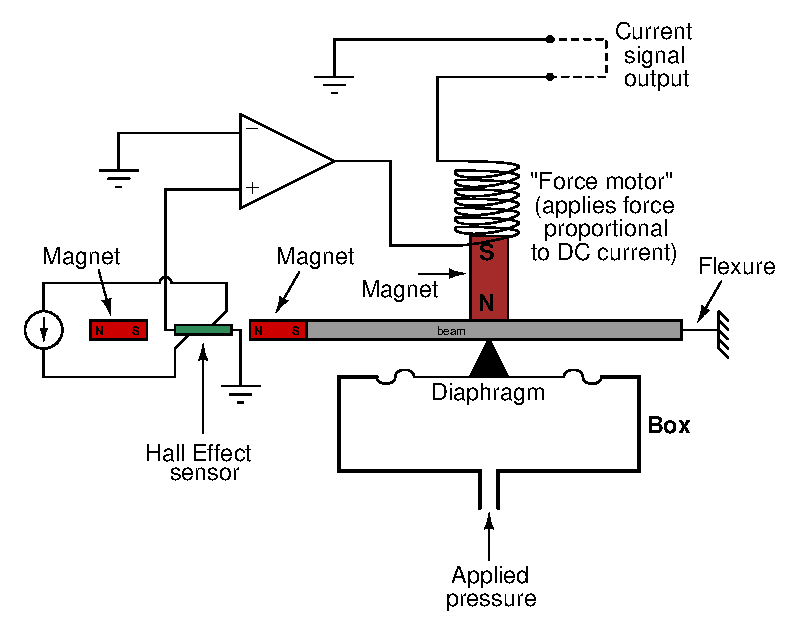
\includegraphics[width=15.5cm]{i00207x01.eps}$$

Forklar følgende med referanse til transmitteren:

\begin{itemize}
\item{} Hva er en \textit{flexure}?
\item{} Hvordan genereres motkraften?
\item{} Hva gjør en \textit{Hall Effect}-sensor?
\item{} Hvordan oppdages ubalanse i kraft?
\item{} Hvordan ville du lagt inn nulljustering i transmitteren?
\item{} Hvordan ville du lagt inn spanjustering i transmitteren?
\end{itemize}

\underbar{file i00207}
%(END_QUESTION)





%(BEGIN_ANSWER)

\noindent
{\bf Delvis svar:}

En \textit{flexure} er en tynn stripe av fjærende materiale, vanligvis fjærstål, laget for å fungere som friksjonsfritt vippepunkt og/eller ledd.  I motsetning til lagre tåler flexures normalt lite vinkelutslag.

\vskip 10pt

\textit{Hall Effect}-sensorer brukes til å detektere magnetfelt.  De genererer en DC-spenning proporsjonal med størrelse og polaritet på magnetfeltet, samt størrelse og retning på en vinkelrett DC-strøm:

$$V_{Hall} = K {IB \over x}$$

$$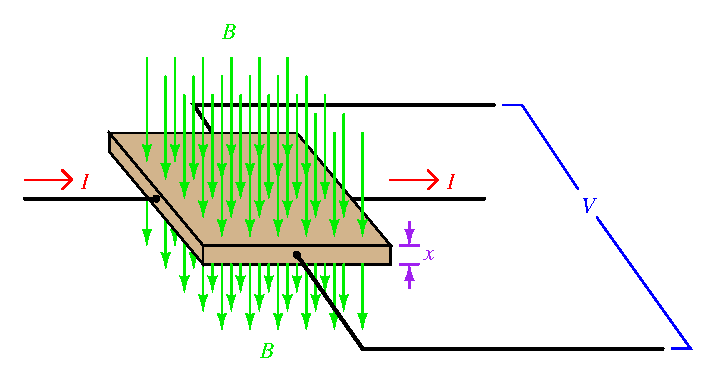
\includegraphics[width=15.5cm]{i00207x02.eps}$$

\filbreak

Driften til Hall-sensoren er ikke alltid intuitiv.  Den er orientert slik at magnetfeltet er parallelt med Hall-spenningsaksen når bjelken er i eksakt nullposisjon.  Når bjelken tipper opp eller ned, vinkles flukslinjene fra ``North''-enden av bjelkemagneten til ``South''-enden av den stasjonære magneten til venstre for sensoren, og passerer sensoren med en tydelig retning opp eller ned avhengig av tippretning:

$$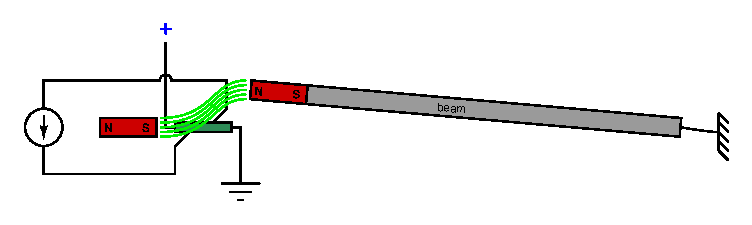
\includegraphics[width=15.5cm]{i00207x03.eps}$$

$$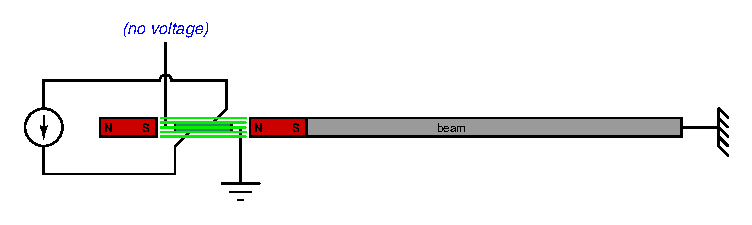
\includegraphics[width=15.5cm]{i00207x05.eps}$$

$$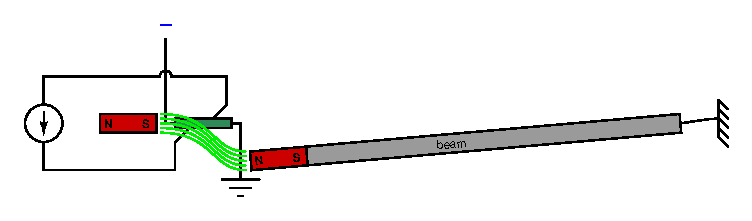
\includegraphics[width=15.5cm]{i00207x04.eps}$$

Dermed indikerer enhver utgangsspenning fra Hall-sensoren en ubalanse mellom membran og kraftmotor.

%(END_ANSWER)





%(BEGIN_NOTES)

Spørsmålene om null og span er ofte de mest interessante.  Minn studentene på at nulljusteringer alltid \textit{adderer} eller \textit{subtraherer}, mens spanjusteringer alltid \textit{multipliserer} eller \textit{dividerer}.

%INDEX% Measurement, pressure: electronic force-balance transmitter

%(END_NOTES)

